\documentclass[a4paper, amsfonts, amssymb, amsmath, reprint, showkeys, nofootinbib, twoside]{revtex4-1}
\usepackage[english]{babel}
\usepackage[utf8]{inputenc}
\usepackage[colorinlistoftodos, color=green!40, prependcaption]{todonotes}
\usepackage[pdftex, pdftitle={Article}, pdfauthor={Author}]{hyperref}
\usepackage{amsthm}
\usepackage{mathtools}
\usepackage{physics}
\usepackage{xcolor}
\usepackage{caption}
\usepackage{hyperref}
\usepackage{multirow}
\usepackage{amsmath}
\usepackage{amssymb}
\usepackage{graphicx}
\graphicspath{Images}
\usepackage[left=23mm,right=13mm,top=35mm,columnsep=15pt]{geometry} 
\usepackage{adjustbox}
\usepackage{placeins}
\usepackage[T1]{fontenc}
\usepackage{float}
%\usepackage{longtable}
\usepackage{csquotes}
\usepackage{refstyle}
\usepackage{lipsum}
\usepackage{booktabs}

\begin{document}

\title{Study of Rutherford Scattering}
\author{Swaroop Ramakant Avarsekar}
\email{swaroop.avarsekar@niser.ac.in}
\affiliation{School of Physical Sciences, National Institute of Science Education and Research, HBNI, Jatni -752050, India}
\date{\today}

\begin{abstract}
Rutherford Scattering was performed to investigate structure of atom, where a beam of $\alpha$ particles are incident on metal and observed that they are scattered at different angles. Most of the particles pass through the metal, some scatter and very few rebound. In experiment replicates the same experiment with smaller time intervals and also calculate the atomic number of Aluminium. We found nuclear charge of aluminium as 23 with relative error of 76.92\%.
\end{abstract}

\keywords{Form factor, Scattering}

\maketitle

\section{Theory}

\begin{figure}[H]
	\centering
	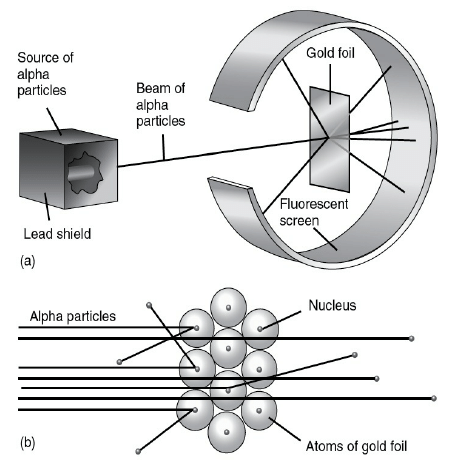
\includegraphics[scale=0.4]{1}
	\caption{Rutherford Scattering experiment}
\end{figure}
Geiger and Marsden under Rutherford performed experiment where collimated $\alpha$ particles were collided with a gold foil and the scintillation were seen on the florescent screen. It was observed that most particles passed through the foil, few scattered at very small angles, and very rarely some back scattered, implying that the most part of the atom is empty, hence nucleus was discovered.

Rutherford calculated the angular distribution of scattering rate N($\theta$), which is defined to be no. of particles scattered during time unit determined interval d$\theta$ around average angle $\theta$.

\begin{equation}
	N(\theta)=N_o.C_f.d_f.\frac{Z^2.e^4}{(8\pi\epsilon_o.E_\alpha)^2 sin^4(\theta/2)}
\end{equation}

$N_o$ is particle rate, $c_f$ is atomic concentration, $d $ is thickness of foil, Z is charge, $E_\alpha$ is energy of $\alpha$ particles.

Regardless of constant, the shape of angular distribution is described as below and shown in fig (2)
\begin{equation}
	f(\theta)=sin^{-4}(\theta/2)
\end{equation} 

\begin{figure}[H]
	\centering
	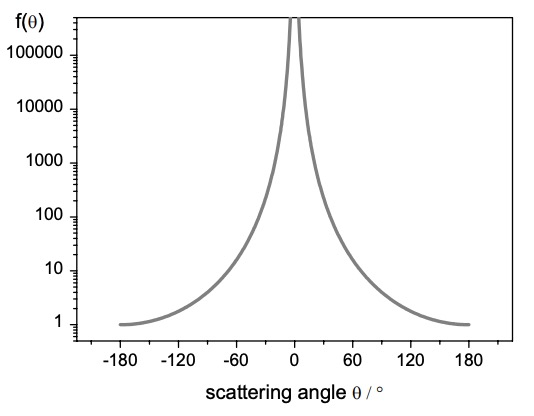
\includegraphics[scale=0.4]{2}
	\caption{Theoretical slope of scattering rate according to equation.}
\end{figure}

Each plane angle $\theta$ corresponds to cone with aperture 2$\theta$. Therefore the angular differential d$\theta$ in 3D should be considered. The spatial scattering rate is given by 
\begin{equation}
	N{\theta}=2\pi. sin(\theta) N_d
\end{equation}

where $N_d=n/t$, n is count and t is time at particular angle.

\begin{figure}[H]
	\centering
	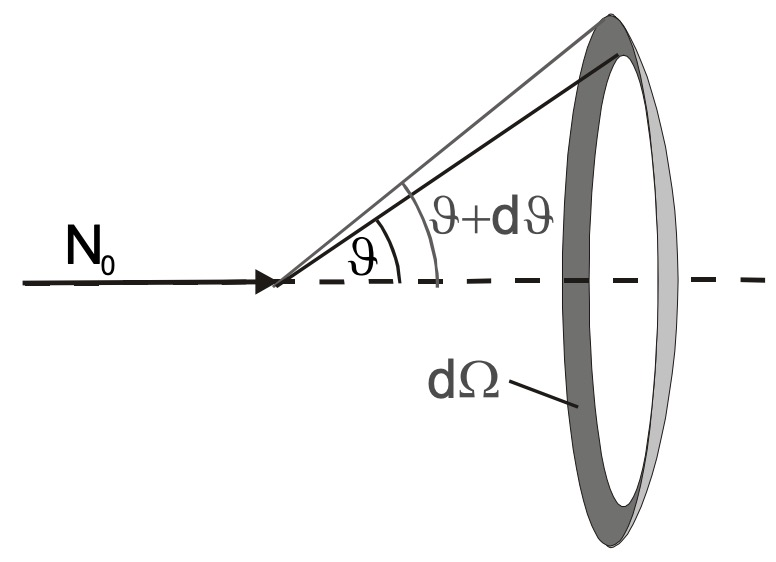
\includegraphics[scale=0.3]{4}
	\caption{Differential scattering cross section in 3D.}
\end{figure}

If we compare the scattering rates between two metal foils 1 and 2, at same angle, then
\begin{equation}
	\frac{N_1}{N_2}=\frac{c_1.d_1.Z^2_1}{c_2.d_2.Z^2_2}
\end{equation}


\section{Experiment}
\begin{figure}[H]
	\centering
	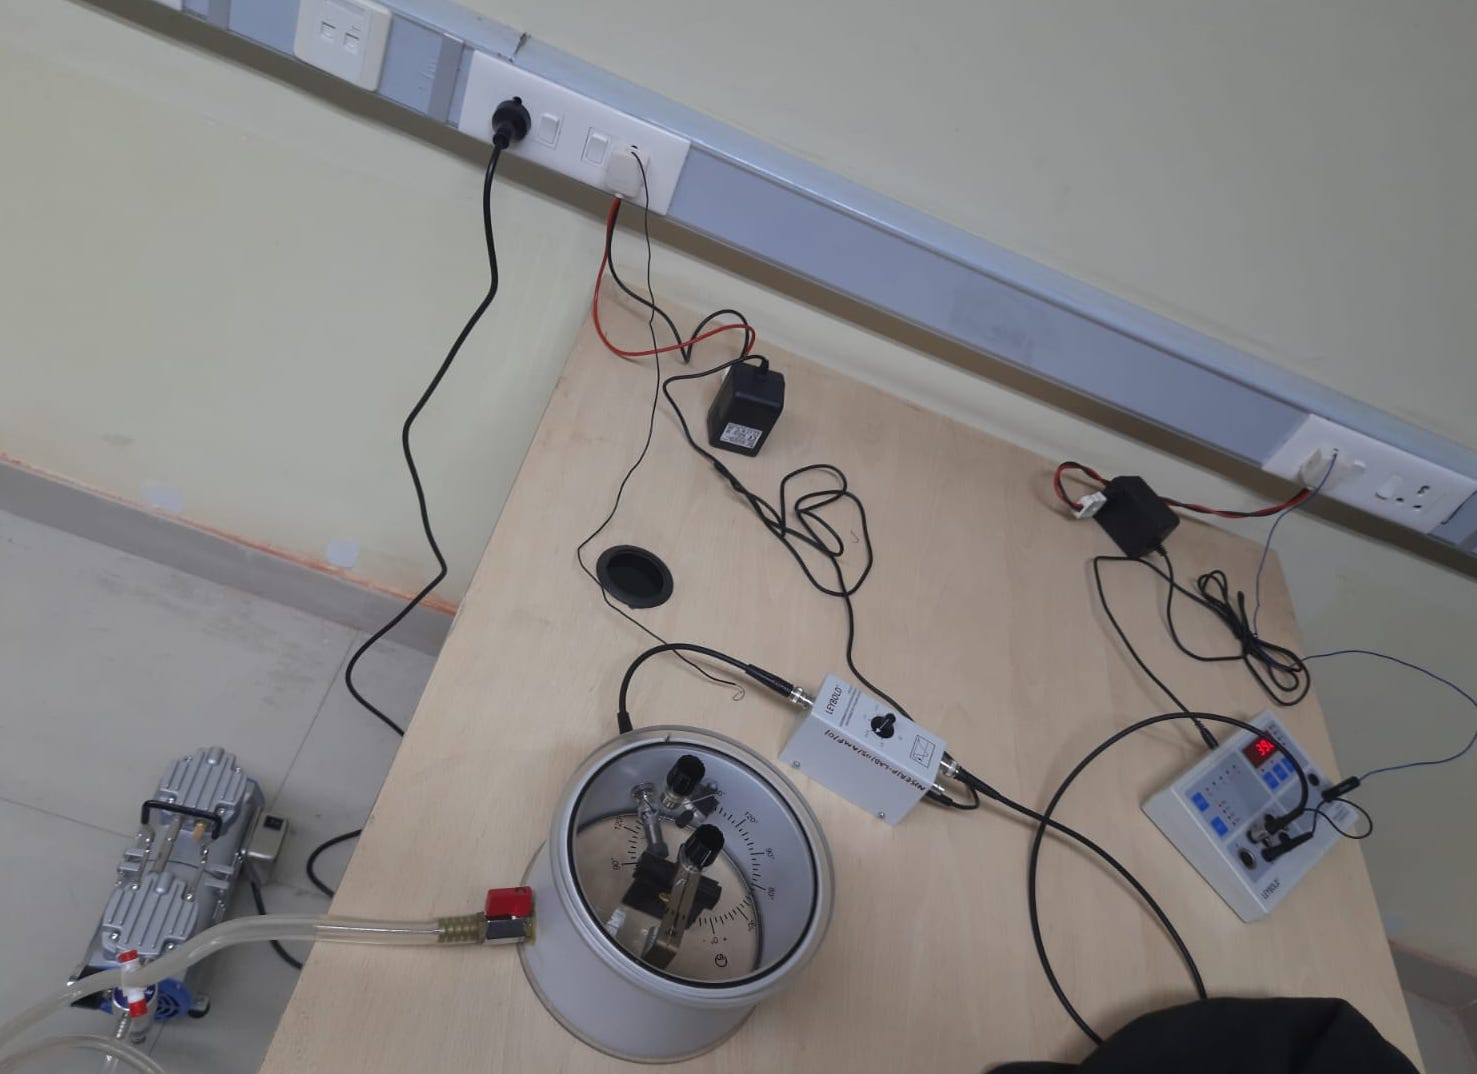
\includegraphics[scale=0.15]{3}
	\caption{Experimental Setup in Laboratory}
\end{figure}


\begin{table}[H]
	\centering
	\caption{Count for gold foil width=5mm}
	\label{tab:my-table}
	\resizebox{\columnwidth}{!}{%
		\begin{tabular}{|c|c|c|c|c|c|}
			\hline
			Time (s) &
			\begin{tabular}[c]{@{}c@{}}Angle \\ (deg)\end{tabular} &
			Count &
			\begin{tabular}[c]{@{}c@{}}Average \\ Count\end{tabular} &
			\begin{tabular}[c]{@{}c@{}}Average \\ Count Rate/s\end{tabular} &
			\begin{tabular}[c]{@{}c@{}}Count rate/s \\ corrected\end{tabular} \\ \hline
			100                  & 5                    & 3314                 & 3314                   & 33.140                  & 18.14798371                  \\ \hline
			100                  & -5                   & 4049                 & 4049                   & 40.490                  & 22.17295898                  \\ \hline
			\multirow{3}{*}{100} & \multirow{3}{*}{10}  & 1824                 & \multirow{3}{*}{1820}  & \multirow{3}{*}{18.200} & \multirow{3}{*}{19.85735895} \\ \cline{3-3}
			&                      & 1781                 &                        &                         &                              \\ \cline{3-3}
			&                      & 1855                 &                        &                         &                              \\ \hline
			\multirow{3}{*}{100} & \multirow{3}{*}{-10} & 3084                 & \multirow{3}{*}{2821}  & \multirow{3}{*}{28.210} & \multirow{3}{*}{30.77890637} \\ \cline{3-3}
			&                      & 2656                 &                        &                         &                              \\ \cline{3-3}
			&                      & 2723                 &                        &                         &                              \\ \hline
			\multirow{2}{*}{100} & \multirow{2}{*}{15}  & 459                  & \multirow{2}{*}{464.5} & \multirow{2}{*}{4.645}  & \multirow{2}{*}{7.553736259} \\ \cline{3-3}
			&                      & 470                  &                        &                         &                              \\ \hline
			\multirow{2}{*}{100} & \multirow{2}{*}{-15} & 977                  & \multirow{2}{*}{972.5} & \multirow{2}{*}{9.725}  & \multirow{2}{*}{15.81487301} \\ \cline{3-3}
			&                      & 968                  &                        &                         &                              \\ \hline
			\multirow{2}{*}{200} & \multirow{2}{*}{20}  & 245                  & \multirow{2}{*}{237.5} & \multirow{2}{*}{1.188}  & \multirow{2}{*}{2.551908928} \\ \cline{3-3}
			&                      & 230                  &                        &                         &                              \\ \hline
			\multirow{2}{*}{200} & \multirow{2}{*}{-20} & 574                  & \multirow{2}{*}{574.5} & \multirow{2}{*}{2.873}  & \multirow{2}{*}{6.172933386} \\ \cline{3-3}
			&                      & 575                  &                        &                         &                              \\ \hline
			\multirow{2}{*}{600} & \multirow{2}{*}{25}  & 485                  & \multirow{2}{*}{377}   & \multirow{2}{*}{0.628}  & \multirow{2}{*}{1.668469329} \\ \cline{3-3}
			&                      & 269                  &                        &                         &                              \\ \hline
			\multirow{2}{*}{600} & \multirow{2}{*}{-25} & 491                  & \multirow{2}{*}{398}   & \multirow{2}{*}{0.663}  & \multirow{2}{*}{1.761407939} \\ \cline{3-3}
			&                      & 305                  &                        &                         &                              \\ \hline
			\multirow{2}{*}{900} & \multirow{2}{*}{30}  & \multirow{2}{*}{246} & \multirow{2}{*}{246}   & \multirow{2}{*}{0.273}  & \multirow{2}{*}{0.858701992} \\
			&                      &                      &                        &                         &                              \\ \hline
			\multirow{2}{*}{900} & \multirow{2}{*}{-30} & \multirow{2}{*}{390} & \multirow{2}{*}{390}   & \multirow{2}{*}{0.433}  & \multirow{2}{*}{1.361356817} \\
			&                      &                      &                        &                         &                              \\ \hline
		\end{tabular}%
	}
\end{table}

\begin{table}[H]
	\centering
	\caption{Count for gold and aluminium foil width=1mm}
	\resizebox{\columnwidth}{!}{%
		\begin{tabular}{|l|l|l|l|l|l|l|}
			\hline
			\begin{tabular}[c]{@{}l@{}}Material \\ (1 mm)\end{tabular} &
			Time (s) &
			\begin{tabular}[c]{@{}l@{}}Angle \\ (deg)\end{tabular} &
			Count &
			\begin{tabular}[c]{@{}l@{}}Average\\  Count\end{tabular} &
			\begin{tabular}[c]{@{}l@{}}Average Count\\  Rate/s\end{tabular} &
			\begin{tabular}[c]{@{}l@{}}Corrected \\ Count Rate/s\end{tabular} \\ \hline
			\multirow{6}{*}{Au} & \multirow{3}{*}{100}  & \multirow{3}{*}{-15} & 32  & \multirow{3}{*}{31.33} & \multirow{3}{*}{0.3133} & \multirow{3}{*}{0.50954518}   \\ \cline{4-4}
			&                       &                      & 27  &                        &                         &                               \\ \cline{4-4}
			&                       &                      & 35  &                        &                         &                               \\ \cline{2-7} 
			& \multirow{3}{*}{100}  & \multirow{3}{*}{15}  & 24  & \multirow{3}{*}{20.67} & \multirow{3}{*}{0.2067} & \multirow{3}{*}{0.3360829911} \\ \cline{4-4}
			&                       &                      & 19  &                        &                         &                               \\ \cline{4-4}
			&                       &                      & 19  &                        &                         &                               \\ \hline
			\multirow{4}{*}{Al} & \multirow{2}{*}{1000} & \multirow{2}{*}{-15} & 85  & \multirow{2}{*}{95.5}  & \multirow{2}{*}{0.0955} & \multirow{2}{*}{0.0155302866}  \\ \cline{4-4}
			&                       &                      & 106 &                        &                         &                               \\ \cline{2-7} 
			& \multirow{2}{*}{1000} & \multirow{2}{*}{15}  & 84 & \multirow{2}{*}{84.5} & \multirow{2}{*}{0.0845} & \multirow{2}{*}{0.06578011447} \\ \cline{4-4}
			&                       &                      & 85 &                        &                         &                               \\ \hline
		\end{tabular}%
	}
\end{table}

From table (1), we plot Scattering angle versus rate and fit it with,
\begin{equation}
	f(\theta)=\frac{A}{sin^4((\theta-B)/2)}
\end{equation}

\begin{figure}[H]
	\centering
	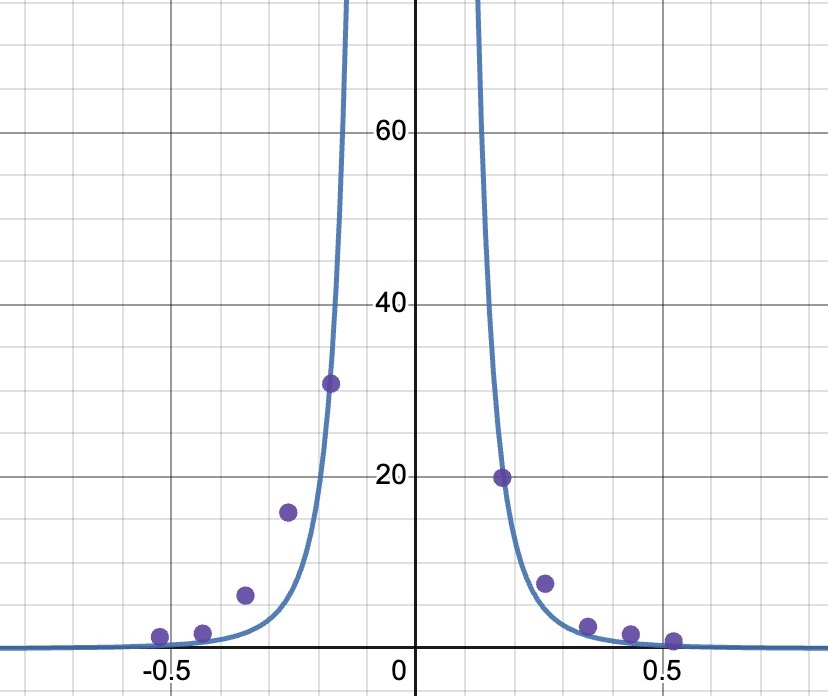
\includegraphics[scale=0.3]{5}
	\caption{Scattering angle versus scattering rate for gold foil of thickness 5 mm. Note that x-axis is scattering angle in radian. y-axis is scattering count.}
\end{figure}

The fit parameters were 0.0015 and -0.0094 for A and B respectively. In the above free fit, angles of -5 and 5 degrees were ignored for better fit to the data. Converting B to degrees gives 0.54 degrees.

To find the nuclear charge, we use equation (4)  with concentration of both metals are equal
\begin{equation}
	Z_{Al}=\sqrt{\frac{N_{Al}.d_{Au}.Z_{Au}^2}{N_{Au}.d_{Al}}}
\end{equation}

The ratio of thickness of gold and aluminium is 0.25.

From calculations, we found that Nuclear charge of Aluminium is 23.24$\approx$23 , with average count rate for Au being 0.26 and 0.09 for Al. The actual value of $Z_{Al}$ is 13.

The relative error is,
\begin{equation}
	\text{Relative Error}=\frac{23-13}{13}\times100\%=76.92\%
\end{equation}


\section{Conclusion}
In this experiment, the angular distributions of scattered particles in Rutherford experiment was studied and fitted with the model. It is seen that most of the counts are read for smaller angles, and as they are increased count value is too low that we had to increase the exposure value to get reasonable count readings. The fit parameters were observed as 0.0015 and -0.0094 respctively. Gold foil was used for different angular counts. In the second part we tried to determine the nuclear charge of aluminium with help of count rate in gold and aluminium. We found nuclear charge of aluminium to be 23 with relative error being 76.92\%. This experiment was unsuccessful in determining nuclear charge as many significant errors have contributed to the experiment.

Maintaining vacuum inside the apparatus is essential part of the experiment, any leakage will perturb the setup and give unnecessary counts. Covering the setup with black cloth is important. In the experiment, the discriminator adjustment plays a crucial role in determining count value, where the value should be neither less nor high. The knob of adjustment of scattering angle was damaged and may have lead to sytematic error and offset. Some electrical fluctuations, inefficient vacuum pump and protection of light contributed to error.


\section{References}
\begin{enumerate}
\item{ SPS NISER Manual}
\item {Desmos-Graphing calculator }
\item\url{{https://www.researchgate.net/figure/Top-Rutherfords-scattering-experiment-with-a-particles-scattering-on-a-gold-foil_fig1_45868627}}
\end{enumerate}

\end{document}